\documentclass{article}
\usepackage[english]{babel}
\usepackage[utf8]{inputenc}
\usepackage{amsmath,amssymb}
\usepackage{parskip}
\usepackage{graphicx}
\usepackage{dsfont}
\usepackage{dsfont}
\usepackage{relsize}
\usepackage{array}
\newcommand{\bigsigma}{\makebox{\Huge\ensuremath{\sigma}}}
\newcommand{\bigpi}{\makebox{\Huge\ensuremath{\Pi}}}
\newcolumntype{C}[1]{>{\centering\let\newline\\\arraybackslash\hspace{0pt}}m{#1}}
\usepackage[top=2.5cm, left=3cm, right=3cm, bottom=4.0cm]{geometry}
\usepackage[table]{xcolor}
\usepackage[utf8]{inputenc}
\usepackage{textcomp}
\usepackage[utf8]{inputenc}
\usepackage{amsmath}
\usepackage{amssymb}
\usepackage{xcolor}
\usepackage{listings}
\usepackage{xstring}
\usepackage{graphicx}
\usepackage[export]{adjustbox}

\definecolor{dkgreen}{rgb}{0,0.6,0}
\definecolor{ltgray}{rgb}{0.5,0.5,0.5}

\makeatletter
\newif\ifcolname
\colnamefalse

\def\keywordcheck{%
\IfStrEq*{\the\lst@token}{select}{\global\colnametrue}{}%
\IfStrEq*{\the\lst@token}{where}{\global\colnametrue}{}%
\IfStrEq*{\the\lst@token}{from}{\global\colnamefalse}{}%
\color{blue}%
}
\def\setidcolor{%
\ifcolname\color{purple}\else\color{black}\fi%
}
\makeatother

\lstset{%
    backgroundcolor=\color{white},
    basicstyle=\footnotesize,
    breakatwhitespace=false,
    breaklines=true,
    captionpos=b,
    commentstyle=\color{dkgreen},
    deletekeywords={...},
    escapeinside={\%*}{*)},
    extendedchars=true,
    frame=single,
    keepspaces=true,
    language=SQL,
    otherkeywords={is},
    morekeywords={*,modify,MODIFY,...},
    keywordstyle=\keywordcheck,
    identifierstyle=\setidcolor,
    numbers=left,
    numbersep=15pt,
    numberstyle=\tiny,
    rulecolor=\color{ltgray},
    showspaces=false,
    showstringspaces=false, 
    showtabs=false,
    stepnumber=1,
    tabsize=4,
    title=\lstname
}

\newcommand{\tablespace}{\\[1.25mm]}
\newcommand\Tstrut{\rule{0pt}{2.6ex}}         % = `top' strut
\newcommand\tstrut{\rule{0pt}{2.0ex}}         % = `top' strut
\newcommand\Bstrut{\rule[-0.9ex]{0pt}{0pt}}   % = `bottom' strut
\title{Assignment-6 CS313}
\author{Shashank P \\ 200010048}
\date{\today}

\begin{document}
\maketitle




\section{Part A}
\subsection{Problem 1}
Extracting and importing the project
into the eclipse workspace using the Handout given with the project.
\begin{figure}[!ht]
  \begin{center}
    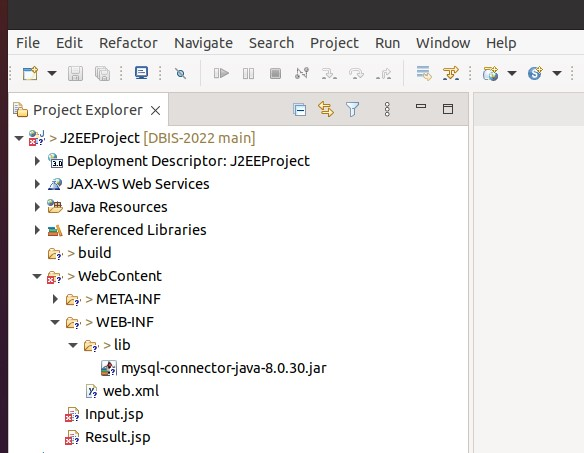
\includegraphics[scale=0.8]{A_1.jpg}
  \caption{Importing the Project}
  \end{center}
\end{figure}

\newpage
\subsection{Problem 2 and 3}
The project has been written using jsp/servlet. It takes student details from the jsp file and adds to
the database using servlet. Then displays the success message on the jsp file.
\begin{figure}[!ht]
  \begin{center}
    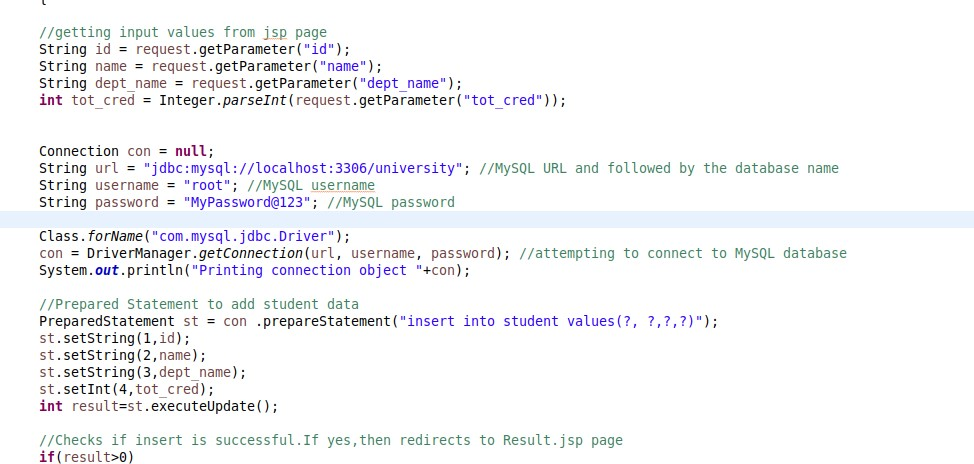
\includegraphics[scale=0.7]{A_2.jpg}
  \caption{Code Modification}
  \end{center}
\end{figure}

The Execution flow is shown in the Figure 3 below.
\begin{figure}[!ht]
  \begin{center}
    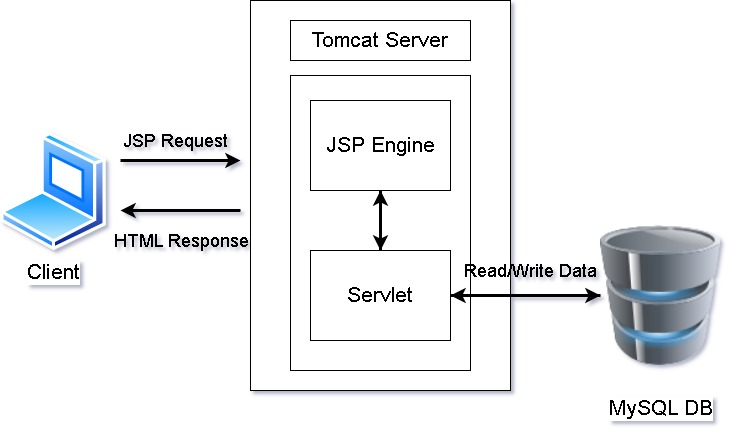
\includegraphics[scale=0.5]{flow.jpg}
  \caption{Execution FLow}
  \end{center}
\end{figure}

\newpage
Adding of student details and the result page is shown in Figure 4 below.
\begin{figure}[!ht]
  \begin{center}
    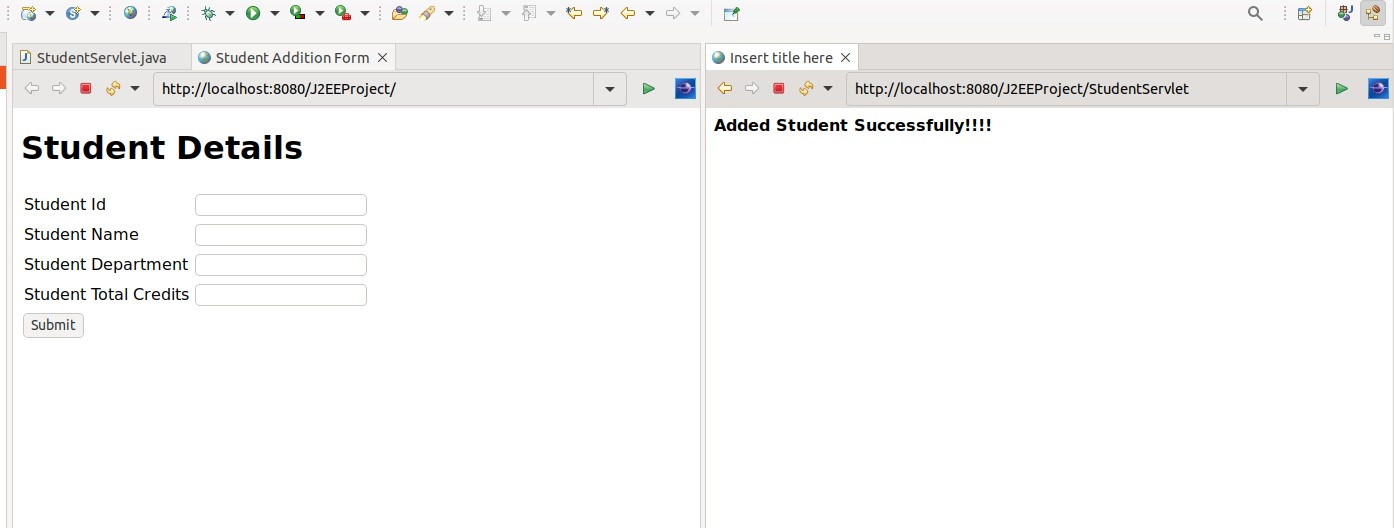
\includegraphics[scale=0.5]{A_3.jpg}
  \caption{Execution}
  \end{center}
\end{figure}


\newpage
\section{Part B}
\subsection{Problem 1}
The objective of this part was to design a tables with appropriate schemas. The Schema is shown below.
\begin{lstlisting}[language=sql]
create database library;
use library;

-- Create Book Table
create table book(
    book_id int,
    title varchar(50) not null,
    category varchar(20),
    author varchar(30) not null,
    primary key(book_id)
);


-- Create Student Table
create table student(
    student_id int,
    name varchar(30) not null,
    dept_name varchar(20),
    year int check(year > 1701 and year < 2100),
    semester varchar(6) check(semester in ('Fall', 'Winter', 'Spring', 'Summer')),
    primary key(student_id)
);

-- Create Issue table
create table issue(
    student_id int not null, 
    book_id int not null, 
    issue_date DATE not null, 
    return_date DATE,
    primary key(student_id, book_id, issue_date),
    foreign key(student_id) references student(student_id) on delete cascade,
    foreign key(book_id) references book(book_id) on delete cascade
);
\end{lstlisting}
\begin{figure}[!ht]
  \begin{center}
    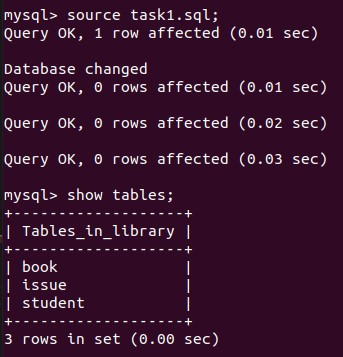
\includegraphics[scale=0.6]{1.jpg}
  \caption{Relevant Tables}
  \end{center}
\end{figure}

\subsection{Problem 2}
Once the tables were created, data was loaded into the tables.
The code for insertion in provided in \textbf{Part-B} folder named, as
\textbf{task2.sql}
\begin{figure}[!ht]
  \begin{center}
    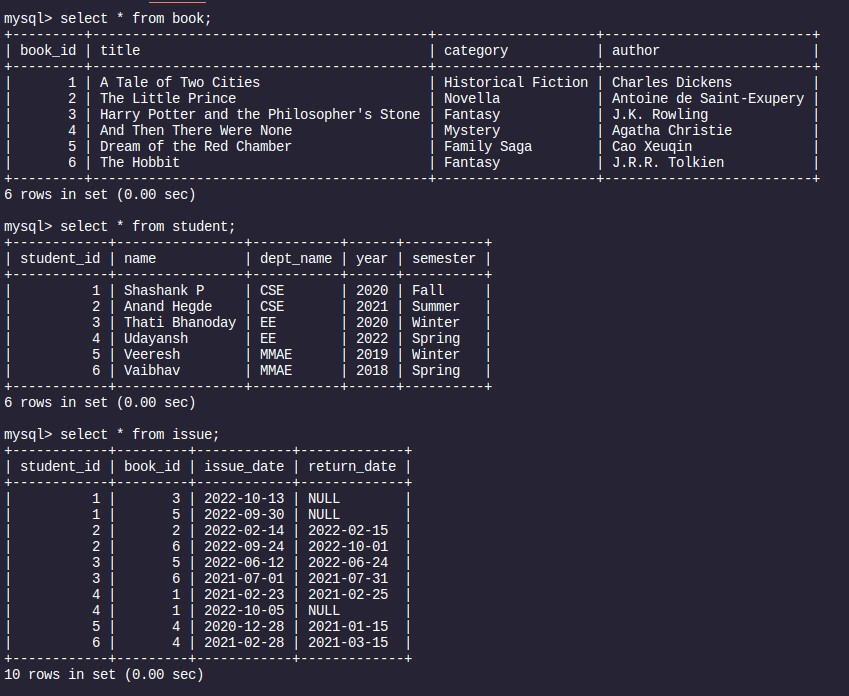
\includegraphics[scale=0.8]{2.jpg}
  \caption{Relevant Tables}
  \end{center}
\end{figure}

\newpage
\subsection{Problem 3}
Then J2EE Project was created with the following specifications
\subsubsection{Home.jsp}
It contains a selection option, to allow the user to choose between \textbf{Adding} or \textbf{Issuing} books.
\begin{figure}[!ht]
  \begin{center}
    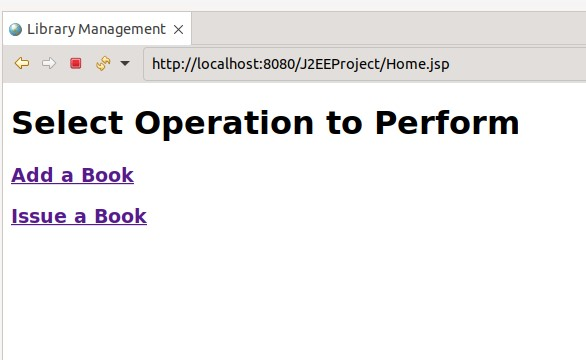
\includegraphics[scale=0.8]{3_home.jpg}
  \caption{Home Page}
  \end{center}
\end{figure}

\subsubsection{Add.jsp}
It allows a user to add new books into the databse by entering relevant information about the books.
On successful addition of a book, a success message is displayed using \textbf{AddResult.jsp}
\begin{figure}[!ht]
  \begin{center}
    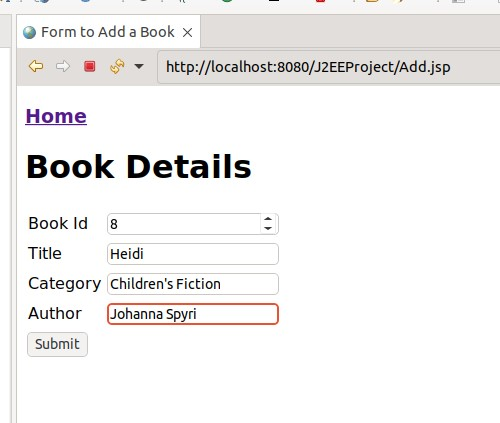
\includegraphics[scale=0.7]{3_add.jpg}
  \caption{Add Page}
  \end{center}
\end{figure}
\begin{figure}[!ht]
  \begin{center}
    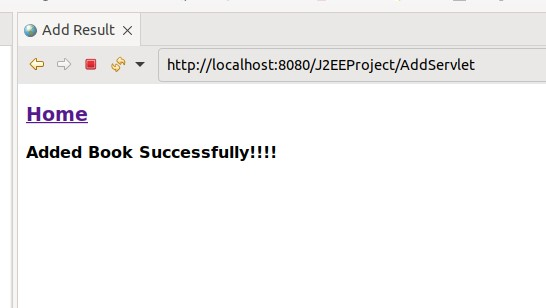
\includegraphics[scale=0.7]{3_add_result.jpg}
  \caption{Add Result}
  \end{center}
\end{figure}

\subsubsection{Issue.jsp}
It allows a user to issue books to students by entering relevant information about the book and the student.
On successful issue of a book, a success message is displayed using \textbf{IssueResult.jsp}
\begin{figure}[!ht]
  \begin{center}
    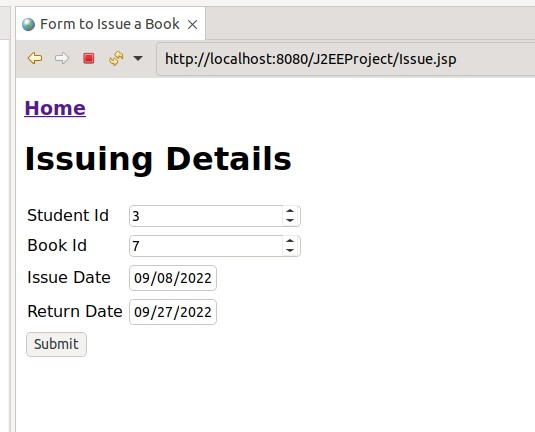
\includegraphics[scale=0.5]{3_issue.jpg}
  \caption{Issue Page}
  \end{center}
\end{figure}
\begin{figure}[!ht]
  \begin{center}
    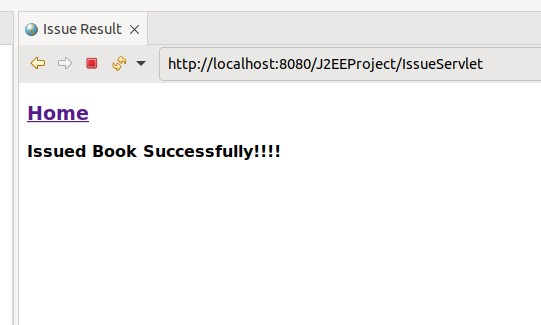
\includegraphics[scale=0.5]{3_issue_result.jpg}
  \caption{Issue Result}
  \end{center}
\end{figure}

\subsubsection{Exception Handling}
During addition of a new book or while issuing of books to students,
several exceptions can occur. These include
\begin{enumerate}
  \item Book already exists.
  \item Book being issued does not exists.
  \item The student to whom the book is issued does not exist.
  \item SQL Exceptions due to connection/environment.
\end{enumerate}
The following images show the handling of different execptions.
\begin{figure}[!ht]
  \begin{center}
    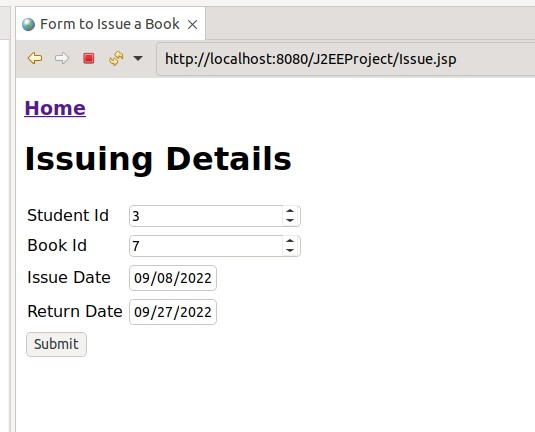
\includegraphics[scale=0.5]{3_issue.jpg}
  \caption{Issue Page}
  \end{center}
\end{figure}
\begin{figure}[!ht]
  \begin{center}
    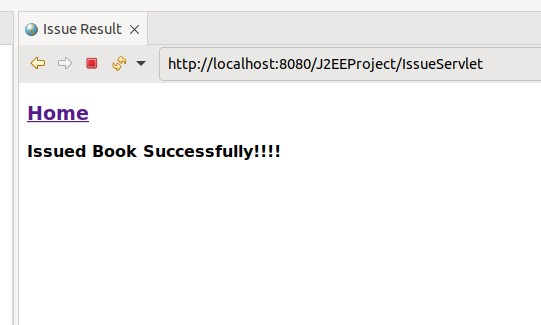
\includegraphics[scale=0.5]{3_issue_result.jpg}
  \caption{Issue Result}
  \end{center}
\end{figure}

\end{document}
